\chapter[EXPERIMENTAL FRAMEWORK]{\huge EXPERIMENTAL FRAMEWORK}
In this chapter is described the validation methodology used with all the classifiers from Vector-based, Spatio-temporal, and Mixed Approaches. Furthermore, it is explained how the data were split and the reasons to do that for the classifier's performance evaluation. Besides, the selected parameters used in all the experiments for each classifier are shown at the end of this chapter.\\

\section{Validation Methodology}
Based on what is mentioned in \cite{brownlee}, Figure \ref{Fig: Validation} shows, inside red squares, the data used by the classifiers in each step of the validation methodology followed in this work. As can be seen, the first step consisted of holding the data of one subject ($S_{m}$) out from the rest to use it later for testing, while the remaining data would be used to train the classifier. This process was done to perform subject-independent experiments similar to \cite{torres2013analisis,torres2016implementing,zhao2015classifying,zhao2013combining}. The reason for performing the experiments in this way was to test if the classifiers could recognize overt and imagined speech from any subject's samples.\\

Then, in the second step, the training data is used to compute scores that would provide an idea of the classifier recognition's capability. These scores were obtained with a k-fold cross-validation process to provide unbiased results. This argument is valid since, on every round of the process, the test fold data were unseen by the time the classifier was trained with the rest data.\\

Therefore, the training scores reported in the next chapter of this work refers to the case when test fold data were used as input to the classifier. Also, the same parameter's initialization was set in all rounds to perform the classifier's training with the same conditions. Besides, a stratified version was used to balance the sample's percent of each class present on the training and test data every round. According to what is mentioned in \cite{forman2010apples}, the main advantage of using stratified k-fold cross-validation is the experimental variance reduction, which makes it easier to identify the best of the methods under consideration.\\

Next, the third step consisted of training again the classifier but with all training data. This step was done to build a final version of the classifier. Finally, the fourth step consisted of testing the trained classifier with the subject data held out at the beginning. Thus, the test scores reported in the next chapter of this work resulted from this final step.\\

\begin{figure}[h!]
	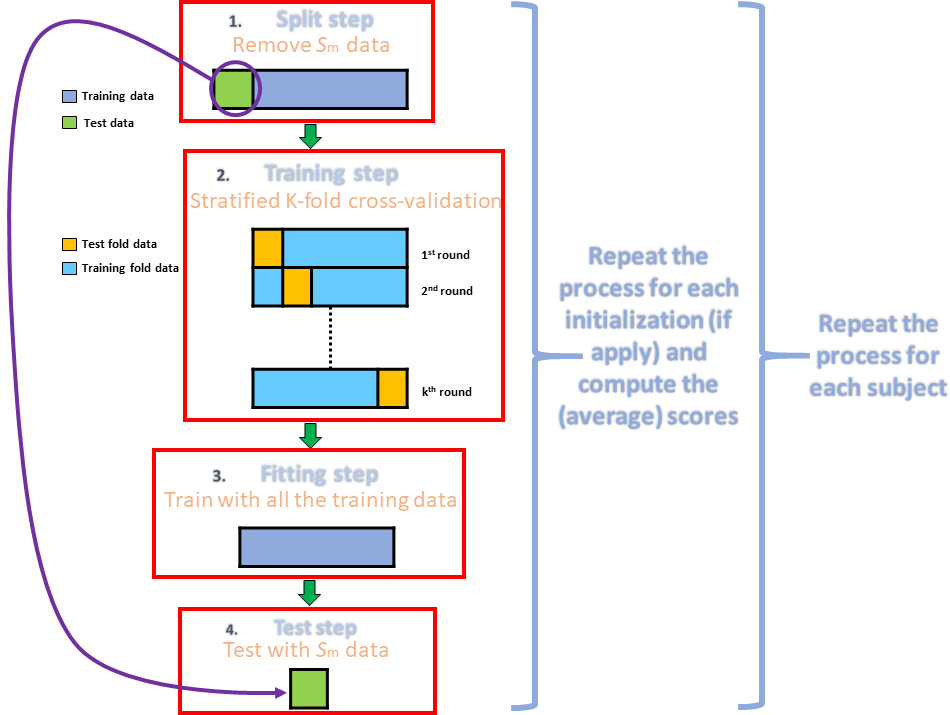
\includegraphics[width=\linewidth]{Figures/Validation.png}
	\centering
	\caption{Data used on each step of the validation methodology followed.}
	\label{Fig: Validation}
\end{figure}

These four steps were repeated several times in case the classifier was sensitive to initial parameters, and the score's averages $\pm$ their standard deviation across the iterations were computed at the end. Besides, the data in step 2 were shuffled to produce different data order on every iteration. Additionally, these steps were repeated by removing data from a different subject in step 1 per time. Thus, the scores reported in this work are identified by whom were the data test.\\

To complement the explanation of this methodology, Algorithm \ref{Algorithm: Validation} shows the details of the followed steps. The matrix $X$ contained the data points of each sample by channel. Then, for this work, $\varsigma$ was conformed by the accuracy, recall, precision, and F1 score names. Besides, the number of subjects $u$ was 5, the number of experiments $n$ (which would cause different classifier's initializations) was set to 20 (if applied), and the number of folds was set to 5. Additionally, the output matrices $S_{f}$ and $S_{t}$ contained, respectively, the scores obtained by using training (test fold) and test data, and from which each row represents which subject data was held out from $X$.\\

Also, the $for$ cycles in steps 2 and 6 represent, respectively, the subject's data selection and the different classifier's parameters initializations per case (second and first bracket in Figure \ref{Fig: Validation}). Table \ref{Table: Validation_Relation} shows the relation between Figure \ref{Fig: Validation} and Algorithm \ref{Algorithm: Validation} steps.\\

\begin{algorithm}
\caption{Validation methodology}
\label{Algorithm: Validation}
\hspace*{\algorithmicindent} \textbf{Input:} \\
\hspace*{\algorithmicindent}\hspace*{\algorithmicindent} $X$: Data samples \\
\hspace*{\algorithmicindent}\hspace*{\algorithmicindent} $\varsigma$: List of score's names to compute \\
\hspace*{\algorithmicindent}\hspace*{\algorithmicindent} $u$: Number of subjects \\
\hspace*{\algorithmicindent}\hspace*{\algorithmicindent} $n$: Number of experiments to perform \\
\hspace*{\algorithmicindent}\hspace*{\algorithmicindent} $f$: Number of folds in the training data \\
\hspace*{\algorithmicindent} \textbf{Output:} \\
\hspace*{\algorithmicindent}\hspace*{\algorithmicindent} $S_{f}$: Training scores (training fold data) \\
\hspace*{\algorithmicindent}\hspace*{\algorithmicindent} $S_{t}$: Test scores (by subject data) \\
\begin{algorithmic}[1]
	\STATE Initialize: matrix $S_{f}$, matrix $S_{t}$
	\FOR{$i=1$ to $u$}{
		\STATE Initialize: list $\varsigma_{f}$, list $\varsigma_{t}$
		\STATE $X_{f} \leftarrow X\setminus\{$data of subject $i\}$
		\STATE $X_{t} \leftarrow \{$data of subject $i\} \in X$
		\FOR{$j=1$ to $n$}{
			\STATE Initialize: classifier's parameters, list $\gamma_{f}$, list $\gamma_{t}$
			\STATE Shuffle $X_{f}$ data
			\FOR{$k=1$ to $f$}{
				\STATE $T \leftarrow X_{f}\setminus \{k$ fold data$\}$
				\STATE $E \leftarrow \{k$ fold data$\} \in X_{c}$
				\STATE Train the classifier with the initial parameters and $T$
				\STATE Test the classifier with $E$, add recognitions to $\gamma_{f}$
			}
			\ENDFOR
			\STATE Train the classifier with the initial values and $X_{f}$
			\STATE Test the classifier with $X_{t}$, add recognitions to $\gamma_{t}$
			\STATE Compute $\varsigma$ scores from $\gamma_{f}$ and $\gamma_{t}$ recognition's lists, then add them to $\varsigma_{f}$ and $\varsigma_{t}$, respectively
		}
		\ENDFOR
		\STATE Compute mean $\varsigma$ scores from $\varsigma_{f}$ and $\varsigma_{t}$, then add them to $S_{f}$ and $S_{t}$, respectively
	}
	\ENDFOR
\end{algorithmic}
\end{algorithm}

\begin{table}[h!]
\caption{Relationship of steps between Figure \ref{Fig: Validation} and Algorithm \ref{Algorithm: Validation}.}
\centering
\begin{tabular}{|c|c|}\hline
	\textbf{Steps Figure \ref{Fig: Validation}}&\textbf{Steps Algorithm \ref{Algorithm: Validation}}\\\hline
	1&3 and 4\\\hline
	2&9 to 14\\\hline
	3&15\\\hline
	4&16\\\hline
\end{tabular}
\label{Table: Validation_Relation}
\end{table}
\pagebreak

Notice that, based on Algorithm \ref{Algorithm: Validation}, the test fold data recognitions were stored in $\gamma_{f}$ and the scores are computed after the $for$ cycle's ending (steps 9 to 14), instead of computing the scores per fold to compute the score averages later. This criterion was chosen due to the conclusions from \cite{forman2010apples}. In \cite{forman2010apples} is mentioned that this criterion avoids biased results, especially under high-class imbalance and using F1 score, which is the case in this work.\\

\section{Parameters' Selection}
Tables \ref{Table: VB_Parameters}, \ref{Table: NeuCube_Parameters}, and \ref{Table: SSN_Parameters} show, respectively, the most important parameters used for the Vector-based approach, NeuCube and SSN classifiers. This means that the scores reported in the next chapter were obtained by using these configurations on each classifier.\\

The $scikit$ learn library, written in Python language, was used to implement the two Vector-based classifiers from this work: MLP and SVM. Also, their parameters (shown in Table \ref{Table: VB_Parameters}) were selected after performing some experiments, which consisted of varying some parameter values and comparing the accuracy obtained with each parameter set following the validation methodology described in the previous section. It is important to note that these experiments were performed by using just some data sets due to the time would consume using all the data configurations.\\

In the case of MLP, these varied parameters were the number of iterations (or epochs) with values of 50, 100, and, 200; as well as the hidden neuron's activation function with the hyperbolic tangent ($tanh$) and the rectified linear unit ($relu$) function. As shown in Table \ref{Table: VB_Parameters}, the configuration that provided the best scores in these experiments was composed of a $tanh$ activation function and 50 iterations.\\

The experiments that used 50 iterations outperformed those with 100 or 200 iterations because, according to the developer site, the $lbfgs$ weight optimization algorithm converges faster with small databases, which is the case in this work. Besides, these configurations were tested with normalized and non-normalized input data, and the best results were obtained by using normalized data.\\

Furthermore, just the kernel type was varied for the SVM with a second-grade polynomial and a radial basis function ($rbf$). As shown in Table \ref{Table: VB_Parameters}, the configuration that provided the best scores was composed of an $rbf$ kernel. Thus, similarly as with MLP, the SVM parameters were tested with normalized and non-normalized data, from which the best results were obtained by using non-normalized data.\\

On the other hand, the NeuCube's parameters, shown in Table \ref{Table: NeuCube_Parameters}, were selected after the grid search was executed for overt and imagined speech samples. In the previous chapter was explained that these grid searches were done over the intervals shown in Table \ref{Table: NeuCube_Gridsearch}. Nonetheless, the grid searches were done with two different parameter sets, which each had the same parameter intervals from Table \ref{Table: NeuCube_Gridsearch} but with their own $\vartheta$ values: \textbf{1.} {0.07, 0.1, 0.13}, and \textbf{2.} {0.05, 0.08, 0.11}. Besides, each grid search was performed twice with different initializations to ensure that the selected parameters were the best for these experiments.\\

\begin{table}[h!]
	\caption{Selected parameters for Vector-based classifiers.}
	\centering
	\begin{tabular}{|l|c|}\hline
		\multicolumn{2}{|c|}{\textbf{Multilayer Perceptron (MLP)}}\\\hline
		Number of hidden neurons (just one layer)&\textit{300}\\\hline
		Activation function of hidden neurons&\textit{tanh}\\\hline
		Weight optimization&\textit{lbfgs}\\\hline
		Regularization term parameter&$1x10^{-4}$\\\hline
		Maximum number of iterations&\textit{50}\\\hline
		\multicolumn{2}{|c|}{\textbf{Support Vector Machine (SVM)}}\\\hline
		Kernel type&rbf\\\hline
		kernel coefficient&\textit{scale}\\\hline
		Tolerance for stopping criterion&$1x10^{-3}$\\\hline
	\end{tabular}
	\label{Table: VB_Parameters}
\end{table}

\begin{table}[h!]
	\caption{Selected parameters for the Neucube.}
	\centering
	\begin{threeparttable}
		\begin{tabular}{|l|}\hline
			\multicolumn{1}{|c|}{\textbf{NeuCube}}\\\hline
			\textbf{SWC}\\\hline
			Radius for candidate connections: \textit{2.5}\\
			Weight values interval: $\pm 0.1$\\
			$r_{+}$: \textit{0.3}\\\hline
			\textbf{LIF}\\\hline
			$\vartheta$: \textit{0.13}, Refractory period: \textit{6}\\\hline
			\textbf{STDP}\\\hline
			Interspike intervals: $\pm 10$\\
			$+A$: 0.001, $-A$: 0.005\\
			Synaptic weight values interval: $\pm 2$\\\hline
			\textbf{deSNN}\\\hline
			$+D$: 0.005, $-D$: 0.001, $\alpha$: \textit{1}, $KNN$: 5\\
			Modulation factor: \textit{0.8}\\\hline
		\end{tabular}
	\end{threeparttable}
	\label{Table: NeuCube_Parameters}
\end{table}

Table \ref{Table: NeuCube_Gridsearch_Values} summarizes the parameters for each grid search performed that provided the best overall accuracy (i.e., the sum of training and test accuracies divided by two). In the cases when overt speech samples were used, the resulting parameters were the same with two different initializations by using the parameter set 1 (highlighted in Table \ref{Table: NeuCube_Gridsearch_Values}).\\

However, the grid searches with different initializations but with the same parameter's intervals varied when imagined speech samples were used. For this reason, classification experiments for imagined speech samples were performed with the two different parameter sets highlighted in Table \ref{Table: NeuCube_Gridsearch_Values} using the $\pm$Bilabial sample's organization.\\

Then, it was selected the parameter's set that provided the best accuracies, which were the same as for overt speech. Due to that, in Table \ref{Table: NeuCube_Parameters} is shown just one parameter set that was used for both: overt and imagined speech.\\
\pagebreak

\begin{table}[h!]
	\centering
	\caption{NeuCube parameter values that provided the best overall accuracy and organized by set used.}
	\scalebox{0.9}{
	\begin{tabular}{|*{10}{c|}}
		\hline
		\textbf{Samples} & \textbf{Set} & \textbf{Initialization} & \boldmath$\vartheta$ & \boldmath$+A$ & \boldmath$-A$ & \boldmath$+D$ & \boldmath$-D$ & \boldmath$r_{+}$ & \textbf{Accuracy} \\\hline
		\multirow{4}{*}{\begin{sideways}\textbf{Overt}\end{sideways}} & \multirow{2}{*}{\textbf{1}} & 1     & \cellcolor{orange}0.13  & \cellcolor{orange}0.001 & \cellcolor{orange}0.005 & \cellcolor{orange}0.005 & \cellcolor{orange}0.001 & \cellcolor{orange}0.3   & 67.15\% \\\cline{3-10}
		&       & 2     & \cellcolor{orange}0.13  & \cellcolor{orange}0.001 & \cellcolor{orange}0.005 & \cellcolor{orange}0.005 & \cellcolor{orange}0.001 & \cellcolor{orange}0.3   & 67.79\% \\\cline{2-10}
		& \multirow{2}{*}{\textbf{2}} & 1     & 0.05  & 0.005 & 0.01  & 0.001 & 0.005 & 0.7   & 66.88\% \\\cline{3-10}
		&       & 2     & 0.05  & 0.001 & 0.01  & 0.001 & 0.01  & 0.3   & 68.17\% \\\hline
		\multirow{4}{*}{\begin{sideways}\textbf{Imagined}\end{sideways}} & \multirow{2}{*}{\textbf{1}} & 1     & \cellcolor{orange}0.13  & \cellcolor{orange}0.001 & \cellcolor{orange}0.001 & \cellcolor{orange}0.01  & \cellcolor{orange}0.005 & \cellcolor{orange}0.3   & 64.29\% \\\cline{3-10}
		&       & 2     & 0.07  & 0.001 & 0.005 & 0.001 & 0.001 & 0.7   & 66.46\% \\\cline{2-10}
		& \multirow{2}{*}{\textbf{2}} & 1     & 0.08  & 0.001 & 0.01  & 0.001 & 0.005 & 0.3   & 64.39\% \\\cline{3-10}
		&       & 2     & 0.05  & 0.001 & 0.001 & 0.001 & 0.01  & 0.7   & 64.29\% \\\hline
	\end{tabular}%
	}
	\label{Table: NeuCube_Gridsearch_Values}%
\end{table}%

\begin{table}[h!]
	\caption{Selected parameters for the SSN.}
	\centering
	\begin{tabular}{|l|}\hline
		\multicolumn{1}{|c|}{\textbf{Single Spiking Neuron (SSN)}}\\\hline
		\textbf{LIF}\\\hline
		$\vartheta$: $[0.1,1.0]$\\
		Refractory period: $[0,6] \in \mathbb{Z}$\\\hline
		\textbf{Izhikevich}\\\hline
		27 behaviours varying:\\
		$a$, $b$, $c$, $d$, $I$\\\hline
		\textbf{Optimization}\\\hline
		Number of generations: \textit{500}\\
		Crossover probability: \textit{0.7}\\
		Weighting factor: \textit{0.1}\\\hline
	\end{tabular}
	\label{Table: SSN_Parameters}
\end{table}

As it has been mentioned in the previous chapter, the SSN has an internal optimization process with a DEA, which tries to find the best parameter configurations based on the constraints stated beforehand. Thus, in Table \ref{Table: SSN_Parameters} are shown the parameters used for the DEA, as well as the interval parameters from both neuron models used with the SSN classifier: LIF and Izhikevich.\\

Notice that the single parameter in Izhikevich model represents the behavior's identifier, which was composed by particular values of the variables $a$, $b$, $c$, $d$, and $I$, These particular values and the behavior's names that the neuron simulates are shown in Table \ref{Table: Izhikevich_behaviors}. Thus, the names and values of the behaviors 0-19 were obtained from \cite{izhikevich2004model} and \cite{izhikevichweb1}, respectively. While,  the names and values of the behaviors 20-26 came from \cite{izhikevich2003simple} and \cite{izhikevichweb2}, respectively.\\

As mentioned in the previous chapter, once the 500 generations of the DEA were performed, the best individual (optimal parameter's values) was selected for the test data. Due to that, in Tables \ref{Table: SSN_Optimal_Overt}, \ref{Table: SSN_Optimal_Imagined}, \ref{Table: SSN_Optimal_DWT}, and \ref{Table: SSN_Optimal_WPT} are shown, respectively, the optimal parameter's values obtained with overt speech, imagined speech, DWT, and WPT samples. Besides, as mentioned before, each subject row represents when such subject was held out from the rest data to test the classifier.\\
\pagebreak

\begin{table}[h!]
	\centering
	\caption{Izhikevich behaviors used in SSN DEA.}
	\scalebox{0.9}{
	\begin{tabular}{|*{3}{c|}}
		\hline
		\textbf{ID} & \textbf{Name}  & \textbf{Values:} \boldmath${a,b,c,d,I}$ \\\hline
		\textbf{0}     &  Tonic spiking & ${0.02, 0.2, -65, 6, 14}$ \\\hline
		\textbf{\textbf{1}}     &  phasic spiking & ${0.02, 0.25, -65, 6, 0.5}$ \\\hline
		\textbf{2}     &  Tonic bursting & ${0.02, 0.2, -50, 2, 15}$ \\\hline
		\textbf{3}     &  Phasic bursting & ${0.02, 0.25, -55, 0.05, 0.6}$ \\\hline
		\textbf{4}     &  Mixed mode & ${0.02, 0.2, -55, 4, 10}$ \\\hline
		\textbf{5}     &  Spike frequency adaptation & ${0.01, 0.2, -65, 8, 30}$ \\\hline
		\textbf{6}     &  Class 1 excitable & ${0.02, -0.1, -55, 6, 0}$ \\\hline
		\textbf{7}     &  Class 2 excitable & ${0.2, 0.26, -65, 0, 1.0}$ \\\hline
		\textbf{8}     &  Spike latency & ${0.02, 0.2, -65, 6, 7}$ \\\hline
		\textbf{9}     &  Subthreshold oscillations & ${0.05, 0.26, -60, 0, 0}$ \\\hline
		\textbf{10}    &  Resonator & ${0.1, 0.26, -60, -1, 0}$ \\\hline
		\textbf{11}    &  Integrator & ${0.02, -0.1, -55, 6, 0}$ \\\hline
		\textbf{12}    &  Rebound spike & ${0.03, 0.25, -60, 4, 0}$ \\\hline
		\textbf{13}    &  Rebound burst & ${0.03, 0.25, -52, 0, 0}$ \\\hline
		\textbf{14}    &  Threshold variability & ${0.03, 0.25, -60, 4, 0}$ \\\hline
		\textbf{15}    &  Bistability & ${1, 1.5, -60, 0, -65}$ \\\hline
		\textbf{16}    &  depolarizing after-potential & ${1, 0.2, -60, -21, 0}$ \\\hline
		\textbf{17}    &  Accomodation & ${0.02, 1.0, -55, 4, 0}$ \\\hline
		\textbf{18}    &  Inhibition-induced spiking & ${-0.02, -1.0, -60, 8, 80}$ \\\hline
		\textbf{19}    &  Inhibition-induced bursting & ${-0.026, -1.0, -45, 0, 80}$ \\\hline
		\textbf{20}    &  Regular spiking neurons (excitatory) & ${0.02, 0.2, -65, 8, 10}$ \\\hline
		\textbf{21}    &  Intrinsically bursting (excitatory) & ${0.02, 0.2, -55, 4, 10}$ \\\hline
		\textbf{22}    &  Chattering (excitatory) & ${0.02, 0.2, -50, 2, 10}$ \\\hline
		\textbf{23}    &  Fast spiking (inhibitory) & ${0.1, 0.2, -65, 2, 10}$ \\\hline
		\textbf{24}    &  Low-threshold spiking (inhibitory) & ${0.02, 0.25, -65, 2, 10}$ \\\hline
		\textbf{25}    &  Inhibitory neurons & ${[0.02, 0.1], [0.2, 0.25], -65, 2.0, [-6.0, 6.0]}$ \\\hline
		\textbf{26}    &  Excitatory neurons & ${0.02, 0.2, [-65, -49]\in \mathbb{Z}, [2, 9], [-15.0, 15.0]}$ \\\hline
	\end{tabular}%
	}
	\label{Table: Izhikevich_behaviors}%
\end{table}%

These parameter's values were used in the classification experiments, which results are shown in the next chapter. Besides, the subscripts 1, 2, and 3 in the variables represent, respectively, when 3 features, 21 features, and EEG signal's data points were used as inputs.\\

Notice that in Tables \ref{Table: SSN_Optimal_DWT}, and \ref{Table: SSN_Optimal_WPT}, subscript 3 is not present, which means that SSN has not been implemented to deal with the additional dimension of these data that represents the wavelet decompositions. Besides, curiously the behavior obtained in all wavelet cases was 13.\\

\begin{table}[h!]
	\centering
	\caption{Optimal SSN parameters obtained from overt speech experiments.}
	\begin{tabular}{|*{11}{c|}}
		\cline{3-11}
		\multicolumn{2}{c|}{\multirow{1}{*}} & \multicolumn{6}{c|}{\textbf{LIF}} & \multicolumn{3}{c|}{\textbf{Izhikevich}} \\\cline{3-11}
		\multicolumn{2}{c|}{\multirow{1}{*}} & \multicolumn{3}{c|}{\textbf{Threshold}} & \multicolumn{3}{c|}{\textbf{Refractory Period}} & \multicolumn{3}{c|}{\textbf{Behavior}} \\\cline{2-11}
		\multicolumn{1}{c|}{\multirow{1}{*}} & \textbf{Subjects} & \multicolumn{1}{c|}{\boldmath$\vartheta_{1}$} & \multicolumn{1}{c|}{\boldmath$\vartheta_{2}$} & \multicolumn{1}{c|}{\boldmath$\vartheta_{3}$} & \multicolumn{1}{c|}{\boldmath$\varrho_{1}$} & \multicolumn{1}{c|}{\boldmath$\varrho_{2}$} & \multicolumn{1}{c|}{\boldmath$\varrho_{3}$} & \multicolumn{1}{c|}{\boldmath$\upsilon_{1}$} & \multicolumn{1}{c|}{\boldmath$\upsilon_{2}$} & \multicolumn{1}{c|}{\boldmath$\upsilon_{3}$} \\\hline
		\multirow{5}{*}{\begin{sideways}\boldmath$\pm$\textbf{Nasal}\end{sideways}} & \boldmath$S_{1}$ & -0.16 & 0.11  & 0.03  & 1     & 4     & 5     & 19    & 19    & 19 \\\cline{2-11}
		& \boldmath$S_{2}$ & -0.13 & 0.66  & 1.05  & 1     & 2     & 4     & 15    & 20    & 4 \\\cline{2-11}
		& \boldmath$S_{3}$ & 0.02  & 0.35  & 0.00  & 1     & 0     & 3     & 15    & 19    & 9 \\\cline{2-11}
		& \boldmath$S_{4}$ & -0.05 & 0.10  & 0.01  & 1     & 5     & 5     & 15    & 18    & 19 \\\cline{2-11}
		& \boldmath$S_{5}$ & -0.09 & 0.29  & 0.00  & 1     & 5     & 6     & 15    & 20    & 15 \\\hline
		\multirow{5}{*}{\begin{sideways}\boldmath$\pm$\textbf{Bilabial}\end{sideways}} & \boldmath$S_{1}$ & 1.00  & 0.87  & 0.75  & 0     & 0    & 0     & 23    & 5     & 0 \\\cline{2-11}
		& \boldmath$S_{2}$ & 0.81  & 1.08  & 0.93  & 0     & 1     & 4     & 23    & 5     & 1 \\\cline{2-11}
		& \boldmath$S_{3}$ & 0.69  & 0.97  & 1.06  & 6     & 0     & 0     & 23    & 5     & 27 \\\cline{2-11}
		& \boldmath$S_{4}$ & 0.74  & 0.85  & 1.00  & 8     & 0     & 0     & 12    & 5     & 1 \\\cline{2-11}
		& \boldmath$S_{5}$ & 0.83  & 1.01  & 1.06  & 6     & 2     & 0    & 27    & 5     & 5 \\\hline
	\end{tabular}%
	\label{Table: SSN_Optimal_Overt}%
\end{table}%

\begin{table}[h!]
	\centering
	\caption{Optimal SSN parameters obtained from imagined speech experiments.}
	\begin{tabular}{|*{11}{c|}}
		\cline{3-11}
		\multicolumn{2}{c|}{\multirow{1}{*}} & \multicolumn{6}{c|}{\textbf{LIF}} & \multicolumn{3}{c|}{\textbf{Izhikevich}} \\\cline{3-11}
		\multicolumn{2}{c|}{\multirow{1}{*}} & \multicolumn{3}{c|}{\textbf{Threshold}} & \multicolumn{3}{c|}{\textbf{Refractory Period}} & \multicolumn{3}{c|}{\textbf{Behavior}} \\\cline{2-11}
		\multicolumn{1}{c|}{\multirow{1}{*}} & \textbf{Subjects} & \multicolumn{1}{c|}{\boldmath$\vartheta_{1}$} & \multicolumn{1}{c|}{\boldmath$\vartheta_{2}$} & \multicolumn{1}{c|}{\boldmath$\vartheta_{3}$} & \multicolumn{1}{c|}{\boldmath$\varrho_{1}$} & \multicolumn{1}{c|}{\boldmath$\varrho_{2}$} & \multicolumn{1}{c|}{\boldmath$\varrho_{3}$} & \multicolumn{1}{c|}{\boldmath$\upsilon_{1}$} & \multicolumn{1}{c|}{\boldmath$\upsilon_{2}$} & \multicolumn{1}{c|}{\boldmath$\upsilon_{3}$} \\\hline
		\multirow{5}{*}{\begin{sideways}\boldmath$\pm$\textbf{Nasal}\end{sideways}} & \boldmath$S_{1}$ & -0.18 & 0.13  & 0.05  & 4     & 0    & 0    & 19    & 0     & 6 \\\cline{2-11}
		& \boldmath$S_{2}$ & 0.07  & 0.03  & 0.62  & 1     & 5     & 5     & 19    & 27    & 6 \\\cline{2-11}
		& \boldmath$S_{3}$ & 0.02  & 0.35  & 0.00  & 1     & 0     & 3     & 15    & 19    & 9 \\\cline{2-11}
		& \boldmath$S_{4}$ & 0.24  & 0.75  & 0.16  & 0     & 5     & 0    & 5     & 19    & 20 \\\cline{2-11}
		& \boldmath$S_{5}$ & 0.25  & 0.03  & 1.02  & 3     & 0    & 4     & 5     & 0     & 0 \\\hline
		\multirow{5}{*}{\begin{sideways}\boldmath$\pm$\textbf{Bilabial}\end{sideways}} & \boldmath$S_{1}$ & 0.71  & 1.04  & 0.07  & 1     & 0     & 6     & 15    & 6     & 15 \\\cline{2-11}
		& \boldmath$S_{2}$ & 0.81  & 0.99  & 0.04  & 0     & 0     & 6     & 15    & 6     & 15 \\\cline{2-11}
		& \boldmath$S_{3}$ & 1.10  & 0.76  & 0.03  & 0     & 0    & 6     & 15    & 5     & 15 \\\cline{2-11}
		& \boldmath$S_{4}$ & 1.18  & 0.70  & 0.05  & 1     & 0     & 6     & 15    & 6     & 15 \\\cline{2-11}
		& \boldmath$S_{5}$ & 1.15  & 0.98  & 0.01  & 0    & 0     & 6     & 15    & 5     & 15 \\\hline
	\end{tabular}%
	\label{Table: SSN_Optimal_Imagined}%
\end{table}%

\begin{table}[h!]
	\centering
	\caption{Optimal SSN parameters obtained from imagined speech experiments using DWT.}
	\begin{tabular}{|*{8}{c|}}
		\cline{3-8}
		\multicolumn{2}{c|}{\multirow{1}{*}} & \multicolumn{4}{c|}{\textbf{LIF}} & \multicolumn{2}{c|}{\textbf{Izhikevich}} \\\cline{3-8}
		\multicolumn{2}{c|}{\multirow{1}{*}} & \multicolumn{2}{c|}{\textbf{Threshold}} & \multicolumn{2}{c|}{\textbf{Refractory Period}} & \multicolumn{2}{c|}{\textbf{Behavior}} \\\cline{2-8}
		\multicolumn{1}{c|}{\multirow{1}{*}} & \textbf{Subjects} & \multicolumn{1}{c|}{\boldmath$\vartheta_{1}$} & \multicolumn{1}{c|}{\boldmath$\vartheta_{2}$} & \multicolumn{1}{c|}{\boldmath$\varrho_{1}$} & \multicolumn{1}{c|}{\boldmath$\varrho_{2}$} & \multicolumn{1}{c|}{\boldmath$\upsilon_{1}$} & \multicolumn{1}{c|}{\boldmath$\upsilon_{2}$} \\\hline
			\multirow{5}{*}{\begin{sideways}\boldmath$\pm$\textbf{Nasal}\end{sideways}} & \boldmath$S_{1}$ & 0.02  & 0.06  & 2     & 6     & 13    & 13 \\\cline{2-8}
			& \boldmath$S_{2}$ & 0.03  & 0.37  & 4     & 2     & 13    & 13 \\\cline{2-8}
			& \boldmath$S_{3}$ & 0.08  & 0.07  & 7     & 3     & 13    & 13 \\\cline{2-8}
			& \boldmath$S_{4}$ & 0.02  & 0.06  & 3     & 0    & 13    & 13 \\\cline{2-8}
			& \boldmath$S_{5}$ & 0.06  & 0.06  & 5     & 2     & 13    & 13 \\\hline
			\multirow{5}{*}{\begin{sideways}\boldmath$\pm$\textbf{Bilabial}\end{sideways}} & \boldmath$S_{1}$ & 0.02  & -0.02 & 4     & 4     & 13    & 13 \\\cline{2-8}
			& \boldmath$S_{2}$ & 0.05  & 0.06  & 5     & 1     & 13    & 13 \\\cline{2-8}
			& \boldmath$S_{3}$ & 0.03  & -0.02 & 5     & 4     & 13    & 13 \\\cline{2-8}
			& \boldmath$S_{4}$ & 0.04  & -0.02 & 6     & 4     & 13    & 13 \\\cline{2-8}
			& \boldmath$S_{5}$ & 0.05  & -0.03 & 6     & 0     & 13    & 13 \\\hline
		\end{tabular}%
		\label{Table: SSN_Optimal_DWT}%
	\end{table}%

\begin{table}[h!]
	\centering
	\caption{Optimal SSN parameters obtained from imagined speech experiments using WPT.}
	\begin{tabular}{|*{8}{c|}}
		\cline{3-8}
		\multicolumn{2}{c|}{\multirow{1}{*}} & \multicolumn{4}{c|}{\textbf{LIF}} & \multicolumn{2}{c|}{\textbf{Izhikevich}} \\\cline{3-8}
		\multicolumn{2}{c|}{\multirow{1}{*}} & \multicolumn{2}{c|}{\textbf{Threshold}} & \multicolumn{2}{c|}{\textbf{Refractory Period}} & \multicolumn{2}{c|}{\textbf{Behavior}} \\\cline{2-8}
		\multicolumn{1}{c|}{\multirow{1}{*}} & \textbf{Subjects} & \multicolumn{1}{c|}{\boldmath$\vartheta_{1}$} & \multicolumn{1}{c|}{\boldmath$\vartheta_{2}$} & \multicolumn{1}{c|}{\boldmath$\varrho_{1}$} & \multicolumn{1}{c|}{\boldmath$\varrho_{2}$} & \multicolumn{1}{c|}{\boldmath$\upsilon_{1}$} & \multicolumn{1}{c|}{\boldmath$\upsilon_{2}$} \\\hline
		\multirow{5}{*}{\begin{sideways}\boldmath$\pm$\textbf{Nasal}\end{sideways}} & \boldmath$S_{1}$ & 0.02  & -0.03 & 4     & 3     & 13    & 13 \\\cline{2-8}
		& \boldmath$S_{2}$ & 0.03  & 0.08  & 2     & 3     & 13    & 13 \\\cline{2-8}
		& \boldmath$S_{3}$ & 0.05  & -0.02 & 5     & 4     & 13    & 13 \\\cline{2-8}
		& \boldmath$S_{4}$ & 0.06  & 0.06  & 5     & 4     & 13    & 13 \\\cline{2-8}
		& \boldmath$S_{5}$ & 0.06  & 0.05  & 5     & 2     & 13    & 13 \\\hline
		\multirow{5}{*}{\begin{sideways}\boldmath$\pm$\textbf{Bilabial}\end{sideways}} & \boldmath$S_{1}$ & 0.04  & -0.03 & 6     & 4     & 13    & 13 \\\cline{2-8}
		& \boldmath$S_{2}$ & 0.06  & 0.07  & 6     & 4     & 13    & 13 \\\cline{2-8}
		& \boldmath$S_{3}$ & 0.03  & 0.06  & 0     & 4     & 13    & 13 \\\cline{2-8}
		& \boldmath$S_{4}$ & 0.05  & 0.07  & 6     & 5     & 13    & 13 \\\cline{2-8}
		& \boldmath$S_{5}$ & 0.04  & 0.09  & 6     & 1     & 13    & 13 \\\hline
	\end{tabular}%
	\label{Table: SSN_Optimal_WPT}%
\end{table}%